
Dans ce chapitre, nous introduisons des concepts de base concernant
l'analyse des s\'eries temporelles. En particulier, nous d\'efinissons
les notions de stationnarit\'e et de fonction d'autocovariance.

\section{Introduction}

%% Nous commen\c{c}ons par d\'efinir ce qu'est une s\'erie temporelle.
%
%\index{S\'erie temporelle}\index{S\'erie chronologique|see{S\'erie temporelle}}
%Une s\'erie temporelle (ou s\'erie chronologique) est un ensemble
%d'observations $x_t$, chacune \'etant enregistr\'ee \`a un instant $t$.
%On rencontre des s\'eries temporelles dans des domaines tr\`es
%vari\'es tels que la m\'edecine, les t\'el\'ecommunications ou l'\'econom\'etrie.

% Notre but, dans cet ouvrage, est de proposer des m\'ethodes permettant
% de mod\'eliser de telles donn\'ees en utilisant un mod\`ele
% math\'ematique appropri\'e afin de pouvoir, par la suite, faire de la
% pr\'ediction. Pour cela, nous proposerons des m\'ethodes permettant
% d'estimer les param\`etres du mod\`ele choisi ainsi que des m\'ethodes
% permettant de tester la validit\'e du mod\`ele propos\'e.


%\paragraph{Exemples de s\'eries temporelles}
% Le paragraphe~\ref{sec:gene} d\'efinit le formalisme probabiliste
% permettant de d\'ecrire les {\em processus al\'eatoires}. Les quelques
% exemples qui suivent illustrent la diversit\'e des situations dans
% lesquelles la mod\'elisation stochastique (ou al\'eatoire) des s\'eries
% temporelles joue un r\^ole important.

Dans la suite, nous proposons de consid\'erer les observations comme
des r\'ealisations d'un processus al\'eatoire $(X_t)_{t\in T}$ dont nous
donnons la d\'efinition dans le paragraphe \ref{sec:gene}. Les quelques
exemples qui suivent illustrent la diversit\'e des situations dans
lesquelles la mod\'elisation stochastique (ou al\'eatoire) des s\'eries
temporelles joue un r\^ole important.
\begin{example}[Trafic internet]
La figure \ref{fig:figtraf} repr\'esente les temps d'inter-arriv\'ees
de paquets TCP, mesur\'es en secondes, sur la passerelle du
laboratoire Lawrence Livermore. La trace repr\'esent\'ee a \'et\'e obtenue
en enregistrant 2 heures de trafic. Pendant cette dur\'ee, environ
1.3 millions de paquets TCP, UDP, etc. ont \'et\'e enregistr\'es.
D'autres s\'eries de ce type peuvent \^{e}tre obtenues sur
\emph{The Internet Traffic Archive},
\emph{http://ita.ee.lbl.gov/}.
%======== FIGURE
\begin{figure}
  \centering
  % Requires \usepackage{graphicx}
  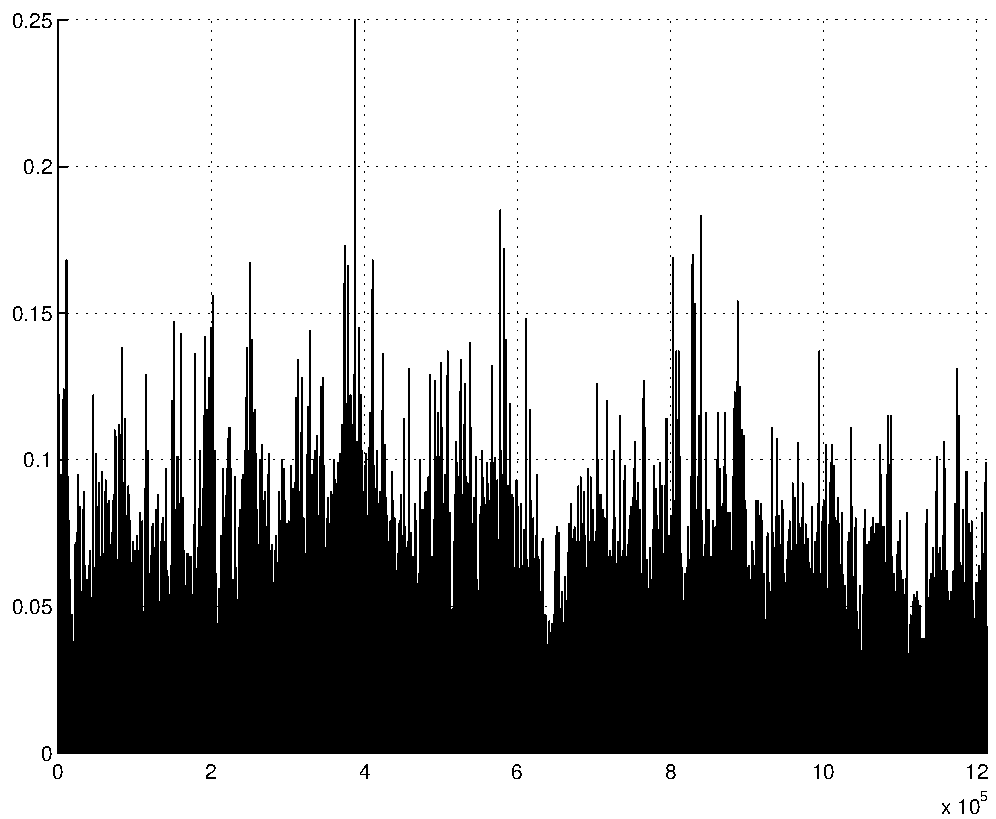
\includegraphics[width=0.5\textwidth]{Figures/lbl_tcp_3}\\
  \caption{Trace de trafic Internet~: temps d'inter-arriv\'ees de paquets TCP.}\label{fig:figtraf}
\end{figure}
\end{example}
\begin{example}[Parole]
La figure \ref{fig:figspeech} repr\'esente un segment de signal
vocal \'echantillonn\'e (la fr\'equence d'\'echantillonnage est de 8000
Hz). Ce segment de signal correspond \`a la r\'ealisation du
phon\`eme \emph{ch} (comme dans \emph{ch}at) qui est un son
dit \emph{fricatif}, c'est-\`a-dire produit par les turbulences du
flot d'air au voisinage d'une constriction (ou resserrement) du
conduit vocal.
%======== FIGURE
\begin{figure}
  \centering
  % Requires \usepackage{graphicx}
  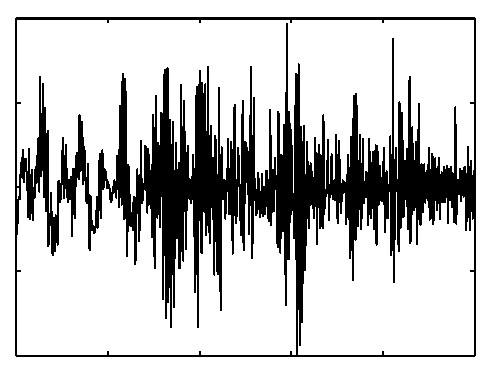
\includegraphics[width=0.5\textwidth]{Figures/phrase}\\
  \caption{Signal de parole \'echantillonn\'e \`a $8000$ Hz~:
 son non vois\'e \emph{ch}.}\label{fig:figspeech}
\end{figure}
\end{example}

\begin{example}[Indice financier]
La figure~\ref{fig:SP} repr\'esente les cours d'ouverture
journaliers de l'indice Standard and Poor 500, du $2$ Janvier
$1990$ au 25 Ao\^ut 2000. l'indice S\&P$500$ est calcul\'e \`a
partir de $500$ actions choisies parmi les valeurs cot\'ees au New
York Stock Exchange (NYSE) et au NASDAQ en fonction de leur
capitalisation, leur liquidit\'e, leur repr\'esentativit\'e dans
diff\'erents secteurs d'activit\'e. Cet indice est obtenu en pond\'erant
le prix des actions par le nombre total d'actions, le poids de
chaque valeur dans l'indice composite \'etant proportionnel \`a la
capitalisation.
%======== FIGURE
\begin{figure}
  \centering
  % Requires \usepackage{graphicx}
  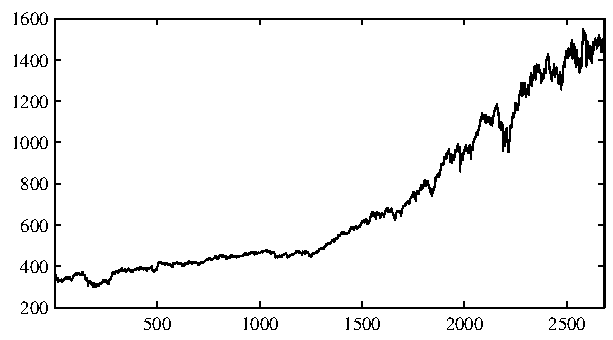
\includegraphics[width=0.5\textwidth]{Figures/SP}\\
  \caption{Cours quotidien d'ouverture de l'indice S\&P$500$~:
 entre Janvier 1990 et Ao\^ut 2000.}\label{fig:SP}
\end{figure}
\end{example}
\begin{example}[Battements cardiaques]
  La figure \ref{fig:figcard1} représente l'évolution, sur une
  durée totale de $900$ secondes, du rythme cardiaque d'un sujet au repos.
  Ce rythme est mesuré en nombre de battements par minute avec un pas d'échantillonnage de $0.5$
  secondes.
\begin{figure}
\label{fig:figcard1}
\centering
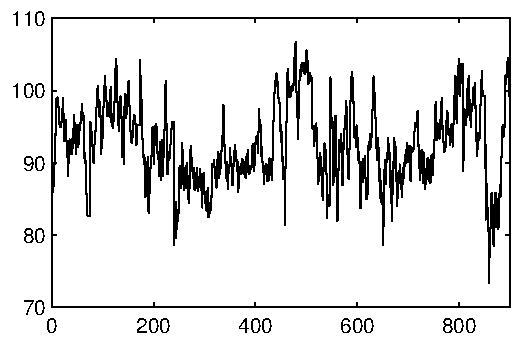
\includegraphics[width=0.5\textwidth]{Figures/hr11839}\\
\caption{Nombre de pulsations par minutes en fonction du temps}
\end{figure}
\end{example}
\section{D\'efinition et construction de la loi d'un processus al\'eatoire}
\label{sec:gene}
%=================================================================
\subsection{Processus al\'eatoire}

\begin{definition}[Processus al\'eatoire]
\index{Processus!Al\'eatoire}
Soient $(\Omega,\cF,\PP)$ un espace de probabilit\'e, $T$ un
ensemble d'indices et $(E,\cE)$ un espace mesurable. On appelle
processus al\'eatoire une famille $(X_t)_{t \in T}$ de v.a. \`a
valeurs dans $(E,\cE)$ index\'ees par $t \in T$.
\end{definition}
Le param\`etre $t$ repr\'esente par exemple le temps. Lorsque $T=
\Zset$ ou $\Nset$, nous dirons que le processus est \`a \emph{temps discret}
et, lorsque $T=\Rset$ ou $\Rset_+$, que le processus est \`a
\emph{temps continu}. Dans la suite, nous nous
int\'eresserons sauf exception aux processus \`a temps
discret avec $T= \Zset$. Quant \`a $(E,\cE)$, nous consid\`ererons
le plus souvent $(\Rset, \cB(\Rset))$ (o\`u $\cB(\Rset)$ est la
tribu bor\'elienne de $\Rset$) ou $(\Rset^d, \cB(\Rset^d))$.
Dans le premier cas, on dira que le processus al\'eatoire est
\emph{scalaire}. Dans le second, nous dirons que le processus est
\emph{vectoriel}.

Notons qu'un processus peut \^{e}tre vu comme une application $X: \Omega
\times T \rightarrow E$, $(\omega,t)\mapsto X_t(\omega)$ telle que, \`a
chaque instant $t \in T$, l'application $\omega \mapsto X_t(\omega)$
est une variable al\'eatoire de $(E,\cE)$.
\begin{definition}[Trajectoire\index{Trajectoire}]
  Pour chaque $\omega\in \Omega$, l'application $t \mapsto
  X_t(\omega)$ est une fonction de $T \rightarrow E$ qui s'appelle la
  \emph{trajectoire} associ\'ee \`a l'\'epreuve $\omega$.
\end{definition}

%==================================================
%==================================================
\subsection{R\'epartitions finies}
%==================================================

Etant donn\'es 2 espaces mesurables $(E_1,\cE_1)$ et $(E_2,\cE_2)$, on d\'efinit l'espace mesurable produit
$(E_1\times E_2,\cE_1\otimes\cE_2)$ o\`u $\times$ d\'esigne le produit cart\'esien usuel des ensembles
et $\otimes$ l'op\'eration correspondante sur les tribus: $\cE_1\otimes\cE_2$ d\'esigne la tribu engendr\'ee par $\{A_1\times A_2,
A_1\in\cE_1: A_2\in\cE_2\}$, ce que l'on \'ecrira
$$
\cE_1\otimes\cE_2=\sigma\{A_1\times A_2: A_1\in\cE_1, A_2\in\cE_2\} \; .
$$
Comme la classe d'ensembles $\{A_1\times A_2: A_1\in\cE_1,
A_2\in\cE_2\}$ est stable par intersection finie, une probabilit\'e sur
$\cE_1\otimes\cE_2$  est \emph{caract\'eris\'ee} par sa restriction \`a
cette classe (voir \cite[Corollaire 6.1]{jacod:protter:2003}).

On d\'efinit de m\^{e}me un espace mesurable produit $(E_1\times\dots\times E_n,\cE_1\otimes\dots\otimes\cE_n)$
\`a partir d'un nombre fini $n$ d'espaces mesurables $(E_t,\cE_t)$,
$t\in T$. Si $T$ n'est pas de cardinal fini, cette d\'efinition se g\'en\'eralise en consid\'erant
 la tribu engendr\'ee par les \emph{cylindres} sur le produit cart\'esien $\prod_{t\in T} E_t$ qui contient l'ensemble des
 familles $(x_t)_{t\in T}$ telles que $x_t\in E_t$ pour tout $t\in T$. Examinons le cas qui nous servira par la suite o\`u
$(E_t,\cE_t)=(E,\cE)$ pour tout $t\in T$. On note alors $E^T=\prod_{t\in T} E$ l'ensemble des trajectoires $(x_t)_{t\in T}$
telles que $x_t\in E$ pour tout $t$, que l'on munit de la tribu engendr\'ee par les cylindres
$$
\cE^{\otimes T}=\sigma\left\{\prod_{t\in I}A_{t}\times E^{T\setminus I} : I\in\mathcal{I},\forall t\in I,\,A_t\in\cE\right\}\;,
$$
o\`u l'on note $\mathcal{I}$ l'ensemble des parties finies de $T$.



%Un \'el\'ement $I$ de $\mathcal{I}$ s'\'ecrit $I = \{ t_1 < t_2 <\cdots < t_n \}$.
Soit $X=(X_t)_{t \in T}$ un processus d\'efini sur  $(\Omega,\cF,\PP)$ \`a
valeurs dans $(E,\cE)$  et $I\in\mathcal{I}$.
On note $\PP_I$ la loi du vecteur al\'eatoire $\{ X_{t}, {t\in I} \}$, c'est-\`a-dire la mesure image  de $\PP$ par ce vecteur~: $\PP_I$ est
la probabilit\'e sur $(E^{I},\cE^{\otimes I})$ d\'efinie par
\begin{equation}
\label{eq:rel1}
\PP_I\left(\prod_{t\in I}A_t\right)
 = \PP\left(X_{t} \in A_t,\,t\in I\right) \eqsp,
\end{equation}
o\`u $A_t$, $t\in T$ sont des \'el\'ements quelconques de la tribu $\cE$. La probabilit\'e $\PP_I$ est
une \emph{probabilit\'e fini-dimensionnelle} ou \emph{r\'epartition finie} du processus $X$.
\begin{definition}
\index{Famille des r\'epartitions finies}
On appelle \emph{famille des r\'epartitions finies} l'ensemble des
r\'epartitions finies $(\PP_I, I \in \mathcal{I})$.
\end{definition}
La sp\'ecification de la mesure $\PP_I$ permet de calculer la
probabilit\'e d'\'ev\'enements de la forme $\PP( \cap_{t \in I} \{
X_t \in A_t \})$ o\`u $\{A_t, t \in I\}$ est une famille d'\'el\'ements de la
tribu $\cE$, ou de mani\`ere \'equivalente, de calculer l'esp\'erance
$\PE {\prod_{t \in I} f_t(X_t) }$ o\`u pour tout $t\in I$, $f_t$ est une
fonction bor\'elienne positive. Soit
$J \subset I$ deux parties finies ordonn\'ees. Soit $\Pi_{I,J}$ la
projection canonique de $E^{I}$ sur $E^{J}$ d\'efinie par
\begin{equation}
\label{eq:rel2} \Pi_{I,J}[ x ] = (x_t)_{t \in J}\quad \text{pour tout}\quad x=(x_t)_{t \in I} \in E^I\;.
\end{equation}
La projection canonique pr\'eserve uniquement les coordonn\'ees du
vecteur appartenant au sous ensemble d'indices $J$.
Par la d\'efinition~(\ref{eq:rel1}), on observe que $\PP_J$ est la mesure image de $\Pi_{I,J}$ d\'efinie sur
l'espace de probabilit\'e $(E^{I},\cE^{\otimes I},\PP_I)$:
\begin{equation}
\label{eq:rel3} \PP_I \circ \Pi_{I,J}^{-1} = \PP_J \;.
\end{equation}
Cette relation
formalise le r\'esultat intuitif que la distribution
fini-dimensionnelle d'un sous-ensemble $J \subset I$ se d\'eduit de
la distribution fini-dimensionnelle $P_I$ en ``int\'egrant'' par rapport aux
variables $X_{t}$ sur l'ensemble des $t$ appartenant au
compl\'ementaire de $J$ dans $I$. Cette propri\'et\'e montre que la
famille des r\'epartitions finies d'un processus est fortement
structur\'ee. En particulier, les r\'epartitions finies doivent, au
moins, v\'erifier les conditions de compatibilit\'e~(\ref{eq:rel3}).
Nous allons voir dans la suite que cette condition est en fait
aussi {\em suffisante}.


Soit $\Pi_I$ la projection canonique de $E^T$ sur $E^I$,
\begin{equation}
\label{eq:projectioncanonique}
\Pi_I( x ) = (x_t)_{t \in I}\quad \text{pour tout}\quad x=(x_t)_{t \in T} \in E^T\;.
\end{equation}
Si $I=\{s\}$ avec $s\in T$, on notera simplement
\begin{equation}
\label{eq:projectioncanoniquesingle}
\Pi_s( x ) =\Pi_{\{s\}}( x )= x_s\quad \text{pour tout}\quad x=(x_t)_{t \in T} \in E^T\;.
\end{equation}

Le th\'eor\`eme suivant montre comment on peut passer d'une famille de
r\'epartitions finies \`a une unique mesure de probabilit\'e sur $(E^T,\cE^{\otimes
  T})$, pourvu que la condition de compatibilit\'e~(\ref{eq:rel3}) soit
satisfaite.

\begin{theorem}[th\'eor\`eme de Kolmogorov]
\label{th:kolmogorov}
%On pose $(E,\cE)=(\Rset^d,\cB(\Rset^d))$ pour $d\geq1$.
Soit $(\nu_I)_{I \in \mathcal{I}}$ une famille de probabilit\'es
index\'ees par l'ensemble des parties finies ordonn\'ees de $T$ telle, que pour tout $I \in \mathcal{I}$,
$\nu_I$ est une probabilit\'e sur $(E^I, \cE^{\otimes I})$. Supposons de plus
que la famille $\{ \nu_I, I \in \mathcal{I} \}$ v\'erifie les conditions
de compatibilit\'e \eqref{eq:rel3}: pour tout $I,J \in \mathcal{I}$, tel que
$I \subset J$, $\nu_I \circ \Pi_{I,J}^{-1} = \nu_J$. Alors, il existe
une unique probabilit\'e $\PP$ sur l'espace mesurable $(E^T,\cE^{\otimes T})$
telle que, pour tout $I \in \mathcal{I}$, $\nu_I = \PP \circ \Pi_I^{-1}$.
\end{theorem}
\begin{proof}\smartqed
Remarquons que la classe des cylindres est une semi-alg\`ebre au sens de
\cite[p.~297]{royden:1988}. On d\'efinit $\PP$ sur cette classe par
$$
\PP\left(\prod_{t\in I}A_{t}\times E^{T\setminus I}\right)=\nu_I \left(\prod_{t\in I}A_{t}\right)\;,
$$
o\`u $I$ d\'ecrit $\cI$ et $A_t\in\cE$ pour tout $t \in I$. La condition
de compatibilit\'e implique que $\PP$ v\'erifie les hypoth\`eses de
\cite[Proposition~9]{royden:1988}. Il s'en suit une extension unique \`a
l'alg\`ebre engendr\'ee par les cylindres, c'est-\`a-dire \`a la plus petite
classe d'ensembles de $E^T$ stable par intersection finie et par
passage au compl\'ementaire contenant les cylindres de $E^T$. Par le
th\'eor\`eme de Carath\'eodory, voir~\cite[Th\'eor\`eme~8]{royden:1988}, on
obtient une unique extension de $\PP$ \`a la tribu $\cE^{\otimes T})$.
\end{proof}

Ceci nous permet de d\'ecrire les r\'epartitions finies d'un processus
donn\'e \`a partir d'une seule probabilit\'e sur $(E^T,\cE^{\otimes T})$, la
\emph{loi} (ou \emph{mesure image}) du processus, d\'efinie comme suit.

\index{Loi}\index{Mesure image|see{Loi}}
\begin{definition}[Loi d'un processus]
\label{def:loi_proc}
Soit $X=(X_t)_{t \in T}$ un processus d\'efini sur  $(\Omega,\cF,\PP)$ \`a valeurs dans $(E,\cE)$. La \emph{mesure image}
$\PP_X$ est l'unique probabilit\'e d\'efinie sur $(E^T,\cE^{\otimes T})$ par $\PP_X\circ\Pi_I^{-1}=\PP_I$ pour tout $I\in\mathcal{I}$, \ie
$$
\PP_X\left(\prod_{t\in I}A_{t} \times E^{T\setminus I}\right) = \PP\left(X_{t}\in A_t,\,t\in I\right)\,
$$
pour tout $(A_t)_{t\in I}\in\cE^I$.
\end{definition}
L'existence et l'unicit\'e de  $\PP_X$ est une cons\'equence du  th\'eor\`eme~\ref{th:kolmogorov}.
Cette loi est donc {\em enti\`erement} d\'etermin\'ee par la donn\'ee des
r\'epartitions finies.

La d\'efinition suivante permet de voir $\PP_X$ comme la probabilit\'e
d'une variable al\'eatoire \`a valeurs dans
$(E^T,\cE^{\otimes T})$. Cette variable al\'eatoire est obtenue comme la
trajectoire du \emph{processus canonique} d\'efini comme suit.

\index{Processus!canonique}
\begin{definition}[Processus canonique]
\label{def:proc_canon}
Soit  $(E,\cE)$ un espace mesurable et $(E^T,\cE^T)$ l'espace mesurable des trajectoires correspondants.
La famille canonique sur $(E^T,\cE^T)$ est la famille des fonctions
mesurables  $(\xi_t)_{t\in T}$ d\'efinies sur
$(E^T,\cE^T)$  \`a valeurs dans  $(E,\cE)$ par $\xi_t(\omega)=\omega_t$ pour tout $\omega=(\omega_t)_{t\in t}\in E^T$.

Quand on munit $(E^T,\cE^T)$ de la \emph{mesure image} $\PP_X$,
on appelle la famille canonique  $(\xi_t)_{t\in T}$ d\'efinies sur $(E^T,\cE^T,\PP_X)$ le \emph{processus canonique} associ\'e
\`a $X$.
\end{definition}

On a suppos\'e jusqu'\`a pr\'esent le processus $X=(X_t)_{t\in T}$ donn\'e.
Le th\'eor\`eme~\ref{th:kolmogorov} peut aussi \^{e}tre utilis\'e pour le
construire, sous la forme d'un processus canonique, comme le montre
l'exemple suivant, puis le paragraphe~\ref{sec:proc-gauss-reels} qui
introduit une classe particuli\`ere de processus~: la classe des
processus gaussiens.

\begin{example}[Suite de v.a. ind\'ependantes]
\label{exple:vaindep}
Soit $(\nu_t)_{t \in T}$ une suite
de probabilit\'es sur $(E,\cE)$. Pour $I\in\mathcal {I}$, on pose
\begin{equation}
\nu_I = \bigotimes_{t\in I} \nu_{t} \;,
\end{equation}
o\`u $\otimes$ d\'esigne le produit tensoriel sur les probabilit\'es (loi du
vecteur \`a composantes ind\'ependantes et de lois
marginales donn\'ees par les $\nu_t$, $t\in I$).
Il est clair que l'on d\'efinit ainsi une famille $(\nu_I)_{I \in
\cI}$ compatible, c'est-\`a-dire, v\'erifiant la condition donn\'ee par
l'\'equation~(\ref{eq:rel3}). Donc, si $\Omega = E^{T}$,
$X_t(\omega)= \omega_t$ et $\cF = \sigma(X_t, t \in T)$, il
existe une unique probabilit\'e $\PP$ sur $(\Omega,\cF)$
telle que $(X_t)_{t \in T}$ soit une suite de v.a.
ind\'ependantes telles que $X_t\sim\nu_t$ pour tout $t\in T$.
\end{example}

\subsection{Processus gaussiens r\'eels}\label{sec:proc-gauss-reels}
%======================================================
Nous introduisons \`a pr\'esent une classe importante de processus al\'eatoires en
mod\'elisation stochastique~: la classe des processus gaussiens.
Rappelons tout d'abord la d\'efinition des variables al\'eatoires
gaussiennes, univari\'ees puis multivari\'ees.

\begin{definition}[Variable al\'eatoire gaussienne r\'eelle]
\index{Variables al\'eatoires!gaussiennes}
 On dit que $X$ est une variable al\'eatoire r\'eelle gaussienne si
 sa loi de probabilit\'e a pour fonction caract\'eristique~:
 $$
   \phi_X(u)=\PE{\rme^{\rmi uX}}=\exp(\rmi \mu u -\sigma^2 u^2/2)
 $$
 o\`u $\mu\in \Rset$ et $\sigma\in\Rset^+$.
\end{definition}
 On en d\'eduit que $\PE{X}=\mu$ et que $\Var{X}=\sigma^2$. Si
$\sigma\neq 0$, la loi poss\`ede une densit\'e de probabilit\'e qui
a pour expression~:
\begin{equation}
  \label{eq:densite-gaussienne-unidim}
 p_X(x)=\frac{1}{\sigma\sqrt{2\pi}}
  \exp\left (-\frac{(x-\mu)^2}{2\sigma^2} \right)\;.
\end{equation}

Si $\sigma=0$, on a alors $X=\mu$ p.s.
La d\'efinition suivante \'etend cette
d\'efinition aux vecteurs al\'eatoires de dimension $n$.

\begin{definition}[Vecteur gaussien r\'eel]
  Un vecteur al\'eatoire r\'eel de dimension $n$
  $[X_1,\dots,X_n]^T$
% \footnote{Dans cet ouvrage, les vecteurs sont par
%     convention identifi\'es sous forme matricielle \`a des vecteurs
%     colonnes et l'exposant $^T$ indique l'op\'erateur de transposition
%     des matrices.}
  est un vecteur gaussien si toute combinaison
  lin\'eaire de $X_1,\dots,X_n$ est une variable al\'eatoire gaussienne
  r\'eelle.
\end{definition}
Notons $\mu$ le vecteur moyenne de $[X_1,\dots,X_n]^T$ et $\Gamma$ sa
matrice de covariance. Par d\'efinition d'un vecteur al\'eatoire gaussien,
pour tout $u\in\Rset^n$, la variable al\'eatoire $Y = \sum_{k=1}^n u_k
X_k=u^TX$ est une variable al\'eatoire r\'eelle gaussienne. Par
cons\'equent, sa loi est compl\`etement d\'etermin\'ee par sa moyenne et sa
variance qui ont pour expressions respectives~:
\[
 \PE { Y }= \sum_{k=1}^n u_k \PE {X_k}=u^T\mu
 \quad \mbox {et} \quad
 \Var{Y}= \sum_{j,k=1}^n u_j u_k \cov(X_j,X_k)=u^T \Gamma u
\]
On en d\'eduit l'expression, en fonction de $\mu$ et de $\Gamma$, de
la fonction caract\'eristique de la loi de probabilit\'e d'un vecteur
gaussien $[X(1),\dots,X(n)]^T$~:
 \begin{equation}
 \label{eq:fcarac_vectgaussien}
 \phi_X(u)=\PE{ \exp( \rmi u^T X) }=\PE{ \exp( \rmi Y) }
 =
 \exp \left ( \rmi u^T \mu - \frac{1}{2}u^T \Gamma u
 \right)
\end{equation}
R\'eciproquement, si un vecteur al\'eatoire $X$ de taille $n$ a une fonction caract\'eristique de
cette forme, on obtient imm\'ediatement que $X$ est un vecteur gaussien en
calculant la fonction caract\'eristique de ses produits scalaires.
Cette propri\'et\'e permet d'obtenir la proposition suivante.
 \begin{proposition}\label{prop:vect_gaussiens}
   La loi d'un vecteur gaussien $X$ de taille $n$ est enti\`erement caract\'eris\'e par son vecteur
   moyenne $\mu$ et sa matrice d'autocovariance $\Gamma$. On notera
$$
X\sim\mathcal{N}_n( \mu, \Gamma) \;.
$$
R\'eciproquement pour tout vecteur
   $\mu\in\Rset^n$ et toute matrice sym\'etrique positive $\Gamma$, il existe un
   vecteur al\'eatoire $X$ tel que $X\sim\mathcal{N}_n( \mu, \Gamma)$.
 \end{proposition}
 \begin{proof}\smartqed
   La premi\`ere partie de l'\'enonc\'e d\'ecoule directement de
   (\ref{eq:fcarac_vectgaussien}).  D\'emontrons maintenant la r\'eciproque. Tout
   d'abord le r\'esultat est vrai pour $n=1$ comme nous l'avons rappel\'e plus haut. On
   passe ais\'ement au cas o\`u $\Gamma$ est diagonale. En effet, notons
   $\sigma_i^2$, $i=1,\dots,n$ ses \'el\'ements diagonaux et
   $\mu=[\mu_1,\dots,\mu_n]^T$. Alors il suffit de prendre $X_1$, \dots ,$X_n$
   ind\'ependants tels que $X_i\sim\mathcal{N}_n( \mu_i, \sigma_i^2)$ pour
   $i=1,\dots,n$. On v\'erifie ais\'ement que $X\sim\mathcal{N}_n( \mu, \Gamma)$ en
   calculant sa fonction caract\'eristique. Pour passer du cas des matrices
   digaonales \`a une matrice $\Gamma$ sym\'etrique
   positive quelconque, on utilise le lemme suivant dont la preuve est laiss\'ee
   \`a titre d'exercice.
   \begin{lemma}
     Soit $X\sim\mathcal{N}_n( \mu, \Gamma)$ avec $\mu\in\Rset^n$ et
      $\Gamma$ matrice sym\'etrique positive $n\times n$. Alors pour toute
      matrice $A$ de taille $p\times n$, on a  $AX\sim\mathcal{N}_n( A\mu,
      A\Gamma A^T)$.
   \end{lemma}
   Pour conclure la preuve de la proposition~\ref{prop:vect_gaussiens}, il
   suffit de remarque que toute matrice sym\'etrique
   positive $\Gamma$ est diagonalisable en base orthonorm\'ee et s'\'ecrit donc
   $\Gamma=U\Sigma U^T$ avec $\Sigma$ matrice diagonale positive et $U$ matrice
   orthogonale. Il suffit alors de prendre $Y\sim\mathcal{N}_n( U^T\mu, \Sigma)$
   et de poser $X=UY$ et le lemme donne $X\sim\mathcal{N}_n( \mu, \Gamma)$
   comme recherch\'e.
\end{proof}

On montre facilement la proposition suivante:

\begin{proposition}\label{prop:vect_gaussiens_indep}
   Soit $X\sim\mathcal{N}_n( \mu, \Gamma)$ avec $\mu\in\Rset^n$ et $\Gamma$
   matrice sym\'etrique positive $n\times n$. Alors $X$ a des composantes
   ind\'ependantes si et seulement si $\Gamma$ est une matrice diagonnale.
 \end{proposition}


En utilisant le m\^{e}me proc\'ed\'e de preuve que pour la
proposition~\ref{prop:vect_gaussiens}, i.e. en consid\'erant le cas $\Gamma$
diagonale puis la diagonalisation de $\Gamma$ pour passer au cas g\'en\'eral, on
obtient aussi le r\'esultat suivant:

 \begin{proposition}\label{prop:vect_gaussiens_densite}
   Soit $X\sim\mathcal{N}_n( \mu, \Gamma)$ avec $\mu\in\Rset^n$ et $\Gamma$
   matrice sym\'etrique positive $n\times n$.  Si $\Gamma$ est de rang plein,
   alors la loi de probabilit\'e de $X$ poss\`ede une densit\'e dans $\Rset^n$ dont
   l'expression est~:
$$
 p_X(x)=\frac{1}{(2\pi)^{n/2}\sqrt{\det(\Gamma)}}
 \exp\left ( -\frac{1}{2}(x-\mu)^T \Gamma^{-1}(x-\mu) \right ),\quad x\in\Rset^n\;.
 $$
\end{proposition}
Dans le cas o\`u $\Gamma$ est de rang $r<n$, c'est \`a dire o\`u $\Gamma$ poss\`ede
 $n-r$ valeurs propres nulles, $X$ se trouve, avec probabilit\'e $1$, dans un
 sous espace affine de dimension $r$ de $\Rset^n$. En effet, il existe alors
 $r-n$ vecteurs $a_i$ formant une famille libre tels que $\cov(a_i^T X) =
 0$ et donc $a_i^T X=a_i^T \mu$ p.s. $X$ n'admet donc \'evidemment pas de
 densit\'e dans ce cas.

Nous \'etendons maintenant la notion de vecteur gaussien \`a celle de
\emph{processus gaussien}.
\begin{definition}[Processus gaussien r\'eel]
\index{Processus!gaussien}
 On dit qu'un processus r\'eel $X= (X_t)_{t \in T}$ est gaussien si,
pour tout ensemble fini d'indices $I=\{t_1, t_2, \cdots,t_n\}$,
$[X_{t_1}, X_{t_2}, \cdots, X_{t_n}]^T$ est un vecteur gaussien.
\end{definition}
Ainsi un vecteur gaussien $[X_1,\dots,X_n]^T$ peut \^{e}tre lui-m\^{e}me vu comme un
processus gaussien $\{X_t, \,t\in \{1,\dots,n\}\}$. Cette d\'efinition
n'a donc un int\'er\^{e}t que dans le cas o\`u $T$ est de cardinal infini.
D'apr\`es~(\ref{eq:fcarac_vectgaussien}), la famille des r\'epartitions finies est
 caract\'eris\'ee par la donn\'ee de la fonction moyenne $\mu:t\in T \mapsto
\mu(t)\in \Rset$ et de la fonction de covariance $\gamma:(t,s)\in(T\times T)
\mapsto \gamma(t,s)\in \Rset$. De plus, pour tout ensemble fini
d'indices $I=\{t_1, t_2, \cdots,t_n\}$, la matrice $\Gamma_I$ d'\'el\'ements
$\Gamma_I(m,k) = \gamma(t_m, t_k)$, o\`u $1 \leq m,k \leq n$, est une matrice
de covariance d'un vecteur al\'eatoire de dimension $n$. Elle est donc
sym\'etrique positive.
R\'eciproquement, donnons nous une fonction $\mu:t\in T \mapsto m(t)\in \Rset$ et
une fonction $\gamma:(t,s)\in(T\times T) \mapsto \gamma(t,s)\in \Rset$ telle
que, pour tout ensemble fini d'indices $I$, la matrice $\Gamma_I$ est
sym\'etrique positive.  On peut alors d\'efinir, pour tout ensemble fini d'indices
$I=\{t_1, t_2, \cdots,t_n\}$, une probabilit\'e gaussienne $\nu_I$ sur $\Rset^n$
par~:
\begin{equation}
\label{eq:rel11} \nu_I \eqdef \mathcal{N}_n( \mu_I, \Gamma_I)
\end{equation}
o\`u $\mu_I= [\mu(t_1), \dots, \mu(t_n)]^T$. La famille $(\nu_I,I \in \cI)$,
ainsi d\'efinie, v\'erifie les conditions de compatibilit\'e et l'on a ainsi \'etabli,
d'apr\`es le th\'eor\`eme \ref{th:kolmogorov}, le r\'esultat suivant~:
\begin{theorem}
  Soit $T$ un ensemble d'indices quelconque, $\mu$ une fonction r\'eelle d\'efinie
  sur $T$ et $\gamma$ une fonction r\'eelle d\'efinie sur $T\times T$ dont toutes
  les restrictions $\Gamma_I$ aux ensembles $I\times I$ avec $I\subseteq T$
  fini forment des matrices sym\'etriques positives. Il existe un espace de
  probabilit\'e $(\Omega,\cF,\PP)$ et un processus al\'eatoire $\{X_t, t
  \in T\}$ gaussien d\'efini sur cet espace v\'erifiant
  \[
  \mu(t)= \PE{ X_t } \quad \mbox{et}\quad \gamma(s,t)= \PE{ (X_s - \mu(s)) (X_t - \mu(t))}\;.
  \]
\end{theorem}
%Attention le r\'esultat ci-dessus est plus subtil qu'il n'y
%para\^{i}t~: si {\em la loi} du processus est bien d\'efinie de mani\`ere unique,
%il existe n\'eanmoins plusieurs mani\`eres de construire des processus ayant cette
%loi. Pour un ensemble $T$ d'indices temporels discret, toutes les
%constructions sont \'equivalentes \`a la construction canonique du
%th\'eor\`eme~\ref{th:kolmogorov}. Pour un ensemble $T$
%non-d\'enombrable (cas des processus \`a temps continu), l'exemple
%ci-dessous montre que l'on cherchera \`a privil\'egier les
%constructions qui garantissent des propri\'et\'es trajectorielles
%suppl\'ementaires comme la continuit\'e des trajectoires.
%\begin{example}[Mouvement brownien]
% Pour mod\'eliser le mouvement d'un grain de pollen dans un liquide, le
% botaniste \'ecossais Brown (circa 1820) a un introduit un processus al\'eatoire
% $X(t)$ \`a valeurs dans $\Rset^2$ ayant des trajectoires ``irr\'eguli\`eres''
% caract\'eris\'ees de la fa\c{c}on suivante~:
%\begin{enumerate}
% \renewcommand\theenumi{(\roman{enumi})}
% \item les accroissements $X(t_2)- X(t_1)$, $\cdots$, $X(t_n)
%-X(t_{n-1})$ sont ind\'ependants (le processus n'a pas de
%``m\'emoire''),
% \item pour tout $h \in \Rset$, et tout $0 \leq
%s < t$, les v.a. $X(t+h) - X(s+h)$ et $X(t) - X(s)$ ont les
%m\^{e}mes lois, et la loi de l'incr\'ement $X(t) - X(s)$ est de
%variance finie $\PE{(X(t)-X(s))^2 } < \infty$,
% \item les trajectoires sont continues.
%\end{enumerate}
%Un tel processus est appel\'e un mouvement brownien. Au d\'ebut du
%XXi\`eme si\`ecle, Louis Bachelier (1900) a observ\'e qu'un tel
%processus \`a valeurs dans $\Rset$ permettait de mod\'eliser le cours
%d'actifs financiers, apr\`es une transformation \'el\'ementaire.
%Albert Einstein (1905), Norbert Wiener (1923) et Paul Levy (1925)
%ont \'et\'e les premiers \`a d\'evelopper une th\'eorie math\'ematique du
%mouvement brownien. Les utilisations d'un tel processus sont
%multiples, et touchent aujourd'hui l'ensemble des domaines des
%sciences de l'ing\'enieur, de l'\'econom\'etrie et de la finance. Nous
%nous int\'eresserons au mouvement Brownien sur $T= \Rset$. Observons
%tout d'abord que, pour $0 \leq t < s$, un tel processus v\'erifie~:
%\begin{equation}
% \label{eq:rel12}
% X(t) - X(s)
% = \sum_{k=1}^{2^n} \left \{
% X(s + 2^{-n}k (t-s)) - X(s + 2^{-n} (k-1) (t-s))
% \right \}
%\end{equation}
%et donc l'accroissement $X(t) - X(s)$ est la somme d'un grand
%nombre de variables al\'eatoires ind\'ependantes de m\^{e}me loi
%(stationnarit\'e des incr\'ements) et de variance tendant vers $0$
%lorsque $n \rightarrow \infty$. Une application directe du
%th\'eor\`eme de la limite centrale montre que $X(t) - X(s)$ suit
%une loi gaussienne.
%\end{example}
%\begin{definition}[Mouvement Brownien]
%\label{def:brownien} Un processus r\'eel $(X(t), t \in \Rset^+)$ est
%un mouvement Brownien issu de $0$ si~:
%\begin{enumerate}
%\renewcommand\theenumi{(\roman{enumi})}
% \item $X(0) = 0$,
% \item Pour tout $t_1 < \cdots < t_n$, les variables al\'eatoires $X(t_2)- X(t_1)$,
%$\cdots$, $X(t_n) - X(t_{n-1})$ sont ind\'ependantes,
% \item pour $t \geq s \geq 0$, l'incr\'ement $(X(t)-X(s))$ est distribu\'e
%suivant une loi gaussienne de moyenne nulle et de variance
%$(t-s)$,
% \item les trajectoires $t \mapsto X(t,\omega)$ sont presque
%s\^urement continues.
%\end{enumerate}
%\end{definition}
%Supposons qu'un tel objet existe. Alors pour tout $ t_1 < \cdots <
%t_n$, on a~:
%\begin{align*}
% X(t_1) &= X(t_1)
% \\
% X(t_2) &= X(t_1) + (X(t_2) - X(t_1)), \cdots
% \\
% X(t_n) &= X(t_1) + (X(t_2) - X(t_1)) + \cdots + (X(t_n) - X(t_{n-1}))
%\end{align*}
%et donc le vecteur $(X(t_1), \cdots, X(t_n))$ est un vecteur
%gaussien, ce qui montre que $X$ est un processus gaussien. Il s'en
%suit que $m(t)=\PE{X(t)} = 0$ et que, pour $0 \leq s < t$, la
%fonction de covariance a pour expression~:
%\[
% \gamma(s,t)
% = \PE{ X(s) X(t)} = \PE{ X(s) (X(s) + (X(t)- X(s))}
% = \PE {X(s)^2} = s
%\]
%et donc $\gamma(s,t)= s \wedge t = \min(t,s)$. Notons que la
%fonction $\gamma(s,t)$ v\'erifie l'\'equation (\ref{eq:rel10}). En
%effet, posant $t_0 = 0$, nous pouvons \'ecrire~:
%\begin{equation}
% \sum_{j,k=1}^n u_j u_k t_j \wedge t_k
% = \sum_{j,k=1}^n
% \left\{ u_j u_k
% \sum_{\ell=1}^{j \wedge k} (t_{\ell} -t_{\ell-1})
% \right \}
% = \sum_{\ell=1}^n
% \left\{ (t_{\ell} - t_{\ell-1})
% \sum_{j=\ell}^n u_{\ell}^2
% \right\} \geq 0
%\end{equation}
%Ceci nous assure l'existence d'un processus gaussien r\'eel $(X(t),
%t \geq 0)$ tel que $\PE{ X(t) } = 0$ et $\PE{X(s) X(t)} = s
%\wedge t$. Pour $0 < s < t$, la variable al\'eatoire $X(t)-X(s)$ est
%distribu\'ee suivant une loi gaussienne de moyenne nulle et de
%variance $t-s$ et, pour $t_1 < t_2 < t_3 < t_4$, $\PE{(X(t_2) -
%X(t_1)) (X(t_4)- X(t_3))}=0$. Et donc, d'apr\`es les propri\'et\'es
%des vecteurs gaussiens, un tel processus v\'erifie les conditions
%(ii) et (iii) de la d\'efinition \ref{def:brownien}. On ne d\'etaille
%pas ici la construction qui permet de montrer qu'il est \'egalement
%possible de v\'erifier la condition (iv).
%=================================================================
%=================================================================
%=================================================================

%\newpage
%======================================================================
%======================================================================
%======================================================================



%==================================================
%==================================================
\section{Stationnarit\'e stricte d'un processus \`a temps discret}
%==================================================
\subsection{D\'efinition}
La notion de stationnarit\'e joue un r\^ole central dans la th\'eorie
des processus al\'eatoires. On distingue ci-dessous deux versions de cette
propri\'et\'e, la \emph{stationnarit\'e stricte} qui fait r\'ef\'erence \`a l'invariance des r\'epartitions finies par translation de l'origine des temps,
et une notion plus faible, la \emph{stationnarit\'e
au second ordre}, qui impose l'invariance par translation des moments
d'ordre un et deux uniquement, lorsque ceux-ci existent.




\begin{definition}[Op\'erateurs  de retard]
\label{def:retard}
On note $\retard$ et l'on appelle \emph{op\'erateur de d\'ecalage} (\emph{Shift}) l'application $E^\Zset\to E^\Zset$ d\'efinie par
$$
\retard(x)= (x_{t-1})_{t\in \Zset}\quad \text{pour tout}\quad x=(x_t)_{t \in \Zset} \in E^\Zset\;.
$$
Pour tout $\tau\in \Zset$, on d\'efinit $\retard^\tau$ par
$$
\retard^\tau(x)= (x_{t-\tau})_{t\in \Zset}\quad \text{pour tout}\quad x=(x_t)_{t \in \Zset} \in E^\Zset\;.
$$
\end{definition}

\begin{definition}[Stationnarit\'e stricte]
\index{Stationnarit\'e!stricte}
Un processus al\'eatoire $X=\{X_t, t\in \Zset \}$ est stationnaire au sens strict si $X$ et $\retard \circ X$ ont m\^{e}me loi, \ie\
 $\PP_{S\circ X}=\PP_X$.
\end{definition}

Par caract\'erisation de la loi image par les r\'epartitions finies, on a  $\PP_{\retard \circ X}=\PP_X$ si et seulement si
$$
\PP_{\retard \circ X}\circ\Pi_I^{-1}=\PP_X\circ\Pi_I^{-1}
$$
pour toute partie finie $I \in \mathcal{I}$.  Or $\PP_{\retard \circ X}\circ\Pi_I^{-1}=\PP_X\circ(\Pi_I\circ \retard)^{-1}$
et $\Pi_I\circ \retard=\Pi_{I-1}$, o\`u $I - 1 = \{ t-1, t \in I \}$.
On en conclut que  $\{X_t, t\in \Zset\}$ est \emph{stationnaire au sens strict} si et seulement si, pour toute partie finie $I \in
\mathcal{I}$,
$$
\PP_I=\PP_{I-1} \; .
$$
On remarque aussi que la stationnarit\'e au sens strict implique que  $X$ et $\retard^\tau\circ X$ ont m\^{e}me loi pour tout $\tau\in \Zset$
et donc aussi $\PP_I=\PP_{I+\tau}$, o\`u $I + \tau = \{ t+\tau, t \in I \}$.

% Killed by oKp on 01/10/01
% \begin{example}[Processus al\'eatoire binaire]
% On consid\`ere le processus al\'eatoire $X= \{ X_n, n \in \Zset \}$ \`a
% valeurs dans l'ensemble $\{0,1\}$. On suppose que, pour tout $n$
% et toute partie finie ordonn\'ee $I = \{ n_1 < \cdots < n_k \}$, les
% variables al\'eatoires $(X_{n_1},X_{n_2},\cdots,X_{n_k})$ sont
% ind\'ependantes, de loi de Bernoulli de param\`etre $\alpha_n$
% \begin{align*}
% & \PP{ X_n = x} = \alpha_n^x (1-\alpha_n)^{1-x}, \ \alpha_n \in [0,1],
% \\
% & \PP{ X_{n_1} = x_1, \cdots, X_{n_k}= x_k}
% = \prod_{i=1}^k \alpha_{n_i}^{x_i} (1-\alpha_{n_i})^{1-x_i}.
% \end{align*}
% Les r\'epartitions finies du processus sont caract\'eris\'ees par la
% donn\'ee de la famille des param\`etres des lois de Bernouilli
% $(\alpha_n)_{n \in \Zset}$. Si le param\`etre $\alpha_n$ des lois de
% Bernouilli est ind\'ependant de $n$, \ie $\alpha_n=\alpha$, nous
% avons, pour tout $n$, tout $I = \{ n_1 < \cdots < n_k \}$
% \[
% \PP { X_{n_1} = x_1, \cdots, X_{n_k}= x_k} = \PP{X_{n_1+n}= x_1,
% \cdots, X_{n_k+n}= x_k} = \prod_{i=1}^k \alpha_{n_i}^{x_i}
% (1-\alpha_{n_i})^{1-x_i}.
% \]
% et donc le processus est stationnaire au sens strict.
% \end{example}
\begin{example}[Processus i.i.d]
\label{exple:iid}
Soit $(Z_t)_{t\in \Zset}$ une suite de variables al\'eatoires \emph{ind\'ependantes et
  identiquement distribu\'ees} (i.i.d) \`a valeurs dans
$\Rset^d$. Alors $(Z_t)_{t\in \Zset}$ est
un processus stationnaire au sens strict, car, pour toute partie finie ordonn\'ee
$I = \{ t_1, < t_2 < \cdots < t_n \}$ et tous bor\'eliens $A_1,\dots,A_n$ de
$\Rset^d$, nous
avons~:
\[
 \PP ( Z_{t_1} \in A_1, \cdots, Z_{t_n} \in A_n)
 =
 \prod_{j=1}^n \PP(Z_0 \in A_j)\;,
\]
qui ne d\'epend pas de $t_1,\dots,t_n$. Notons que d'apr\`es \Cref{exple:vaindep}, pour toute probabilit\'e $\nu$ sur $\Rset^d$, on
sait construire un processus $(Z_t)$ i.i.d. de \emph{loi marginale} \index{Loi marginale}
$\nu$, c'est-\`a-dire tel que $Z_t\sim \nu$ pour tout $t\in \Zset$.
\end{example}

\begin{example}[Transformation d'un processus i.i.d.]
\label{exple:trans_iid}
Soit $Z$ un processus i.i.d. (voir \Cref{exple:iid}).
Soient $k$ un entier et $g$ une fonction bor\'elienne de $\Rset^k$
dans $\Rset$. On peut v\'erifier que le processus al\'eatoire
$(X_t)_{t\in\Zset}$ d\'efini par
\[
 X_t= g(Z(t), Z(t-1), \cdots, Z(t-k+1))
\]
est encore un processus al\'eatoire stationnaire au sens strict.  Par contre, ce
processus obtenu par transformation n'est plus i.i.d dans la mesure o\`u, d\`es que
$k \geq 1$, $X_t, X_{t+1}, \dots, X_{t+k-1}$ ont bien la m\^{e}me distribution
marginale mais sont, en g\'en\'eral, d\'ependants car fonctions de variables
al\'eatoires communes. Un tel processus est dit $k$-d\'ependant car pour $\tau \geq k$,
$(X_s)_{s\leq t}$ et $(X_s)_{s\geq t+\tau}$ sont ind\'ependants pour tout $t$. Les processus $m$-d\'ependants
peuvent \^{e}tre utilis\'es pour approcher une grande classe de processus d\'ependants
afin d'\'etudier le comportement asymptotique de statistiques usuelles telles que
la moyenne empirique.  \index{Processus!$m$-d\'ependant}
\end{example}


\subsection{Transformations pr\'eservant la stationnarit\'e}

On pose $E=\Cset^d$ et $\cE=\cB(\Cset^d)$ pour un entier
$d\geq1$.




\begin{definition}[Filtrage]
  Soit $\phi$ une application mesurable de $(E^\Zset,\cE^{\otimes \Zset})$
  dans $(F^\Zset,\cF^{\otimes \Zset})$ et $X=(X_t)_{t\in \Zset}$ un processus \`a valeurs dans $(E,\cE)$.
  On appelle \emph{filtr\'e} du processus $X$ par la transformation $\phi$ le
  processus $Y=(Y_t)_{t\in \Zset}$ \`a valeurs dans $(F,\cF)$ d\'efini par
  $Y=\phi\circ X$, c'est-\`a-dire $Y_t=\Pi_t(\phi( X))$ pour tout $t\in
  \Zset$, o\`u $\Pi_t$ est d\'efini par~(\ref{eq:projectioncanoniquesingle}). Si
  $\phi$ est une application lin\'eaire, on parlera de \emph{filtrage lin\'eaire}.
\end{definition}

L'exemple~\ref{exple:trans_iid} est un exemple de filtrage (en g\'en\'eral
non--lin\'eaire, \`a moins que $g$ soit une forme lin\'eaire).  La transformation
associ\'ee \`a cet exemple est l'application $\phi:\Rset^\Zset\to\Rset^\Zset$
d\'efinie par
$$
\phi\big((x_t)_{t\in\Zset}\big)=
\big(g(x_t,x_{t-1},\dots,x_{t-k+1})\big)_{t\in\Zset}\;.
$$


\begin{example}[D\'ecalage]
\label{exple:decalage}
  Un exemple fondamental de filtrage lin\'eaire de processus est obtenu en
  prenant $\phi=S$ o\`u $S$ est l'op\'erateur de d\'ecalage de la
  d\'efinition~\ref{def:retard}. Dans ce cas $Y_t=X_{t+1}$ pour tout $t\in \Zset$.
\end{example}


\begin{example}[Filtre \`a r\'eponse impulsionnelle finie (RIF)]
\label{exple:rif}
  Soient $n\geq1$ et $t_1<\dots < t_n$ des \'el\'ements de $\Zset$ et
  $\alpha_1,\dots,\alpha_n\in E$. Alors $\sum_i\alpha_i S^{-t_i}$ d\'efinit un
  filtrage lin\'eaire pour n'importe quel processus $X=(X_t)_{t\in \Zset}$ pour
  lequel la sortie est donn\'ee par
$$
Y_t=\sum_{i=1}^n\alpha_i X_{t-t_i},\quad t\in \Zset \; .
$$
\end{example}
\begin{example}[Diff\'erentiation]
\label{exple:diff}
Un cas particulier de l'exemple pr\'ec\'edent est donn\'e par l'\emph{op\'erateur de diff\'erentiation} $I-S^{-1}$ o\`u $I$ d\'enote l'op\'erateur
identit\'e. Le processus obtenu en sortie s'\'ecrit
$$
Y_t=X_t-X_{t-1},\quad t\in \Zset \; .
$$
On pourra it\'erer l'op\'erateur de diff\'erentiation, ainsi $Y=(I-S^{-1})^kX$ est
donn\'ee par
$$
Y_t=\sum_{j=0}^k {{k}\choose{j}} (-1)^j X_{t-j} ,\quad t\in \Zset \; .
$$
\end{example}
\begin{example}[Retournement du temps]
\label{exple:time_reversion}
Etant donn\'e un processus  $X=\{X_t, t\in \Zset\}$, on appellera \emph{processus retourn\'e} le processus obtenu par
\emph{retournement du temps} d\'efini par
$$
Y_t=X_{-t},\quad t\in \Zset \; .
$$
\end{example}
\begin{example}[Int\'egration]
\label{exple:time_integration}
  Etant donn\'e un processus $X=(X_t)_{t\in \Zset}$ qui v\'erifie
  $\sum_{t=-\infty}^0|X_t|<\infty$ p.s., on appellera \emph{processus int\'egr\'e}
  le processus d\'efini par
$$
Y_t=\sum_{s=0}^\infty X_{t-s},\quad t\in \Zset \; .
$$
Contrairement aux exemples pr\'ec\'edents, l'application $\phi$ qui d\'efinit ce
filtrage doit \^{e}tre d\'efinie avec quelques pr\'ecautions. Il faut en effet tout
d'abord d\'efinir $\phi$ sur
$$
A=\left\{x=(x_t)_{t\in \Zset}\in E^\Zset~:~\sum_{t=-\infty}^0|x_t|<\infty\right\}\;,
$$
par $\phi(x)=\sum_{s=0}^\infty x_{t-s}$. Comme $A$ est un espace vectoriel, on
peut prolonger $\phi$ lin\'eairement sur $(E^\Zset,\cE^{\otimes \Zset})$. Le
point important est que ce filtrage ne sera appliqu\'e \`a $X$ que sous l'hypoth\`ese
$\sum_{t=-\infty}^0|X_t|<\infty$ p.s. et que ce prolongement est donc d\'efini de
fa\c{c}on \emph{quelconque}.
\end{example}

On remarque que dans tous les exemples pr\'ec\'edents les op\'erateurs introduits
pr\'eservent la stationnarit\'e stricte,
c'est-\`a-dire, si $X$ est strictement stationnaire alors $Y$ l'est
aussi. Il est facile de construire des
filtrages lin\'eaires qui ne pr\'eserve pas la stationnarit\'e stricte, par exemple,
$y=\phi(x)$ avec $y_t=x_t$ pour $t$ pair et $y_t=x_t+1$ pour $t$ impaire. Une propri\'et\'e plus
forte que la conservation de la stationnarit\'e est donn\'ee par la d\'efinition
suivante.

\begin{definition}
  Un filtrage lin\'eaire est \emph{invariant par translation} s'il commute avec
  $S$: $\phi\circ S=S\circ \phi$.
\end{definition}

Cette propri\'et\'e implique la pr\'eservation de la stationnarit\'e mais ne lui est
pas \'equivalente. Le retournement du temps est en effet un exemple de filtrage
qui ne commute pas avec $S$ puisque dans ce cas on a $\phi\circ S=S^{-1}\circ
\phi$.  En revanche tous les autres exemples ci-dessus satisfont la propri\'et\'e
d'invariance par translation.

\begin{remark}
\label{rem:FiltrageInvTrans}
Un filtrage $\phi$ \emph{invariant par translation} est enti\`erement
d\'etermin\'e par sa composition avec sa composition avec la projection canonique
$\Pi_0$,
voir~(\ref{eq:projectioncanoniquesingle}). En effet, notons
$\phi_0=\Pi_0\circ\phi$. Alors pour tout $s\in \Zset$, $\Pi_s\circ\phi=
\Pi_0\circ S^{s}\circ\phi=\Pi_0\circ\phi\circ S^{s}$. Il suffit enfin
d'observer que pour tout $x\in E^\Zset$, $\phi(x)$ est la suite
$(\pi_s\circ\phi)_{s\in \Zset}$.
\end{remark}









%%% Local Variables:
%%% mode: latex
%%% ispell-local-dictionary: "francais"
%%% TeX-master: "../monographie-serietemporelle"
%%% End:

